\section{Documentazione software MATLAB}
In questo paragrafo viene descritta l'implementazione del \textit{filtro di Kalman} come sistema dinamico ed il task implementato dal nostro gruppo in ambiente di programmazione \textit{MATLAB}, usando l'approccio della programmazione orientata agli oggetti.

\subsection{\texttt{sistema.m}}
\textit{MATLAB} presenta già un'implementazione dei modelli di sistemi dinamici lineari ma si è preferito realizzarne una nuova implementazione che considerasse anche gli errori di processo e di misura in modo da rispettare le ipotesi del problema.

In particolare nel file \texttt{sistema.m} viene implementata la \textit{classe} dei sistemi dinamici stocastici che utilizzeremo.

Per semplicità abbiamo implementato soltanto sistemi tempo invarianti, per cui tutte le matrici che definiscono il sistema sono costanti.
\subsubsection{Proprietà}
Le proprietà di cui dispongono gli oggetti di questa classe sono :
\begin{lstlisting}[frame=single]
classdef sistema < handle
%SISTEMA 
%Classe che descrive un sistema dinamico lineare tempo invariante

	properties (Access = protected)
		A,B,C,D,W,Q,R,x;    %A,B,C,D matrici del sistema
		% W matrice di guadagno del rumore di processo
		% Q matrice di covarianza del rumore di processo
		% R matrice di covarianza del rumore di misura
		n,m,p,q;      %n dim stato, m dim ingresso, p dim uscita, q dim rumore di processo
		u;       %ultimo ingresso ricevuto
	end
\end{lstlisting}
I metodi implementati sono il costruttore dell'oggetto che va ad inizializzarlo e le due equazioni di evoluzione dello stato interno e di uscita.\\
\newpage
\subsubsection{Costruttore}
La creazione dell'oggetto \texttt{sistema} avviene tramite l'inizializzazione dei suoi parametri:
\begin{lstlisting}[frame=single]
function obj = sistema(A,B,C,D,W,Q,R,x0)
\end{lstlisting}
Al costruttore vanno passate tutte le matrici relative al caso preso in analisi (comprese le covarianze) ed il suo stato iniziale.\\
Al suo interno vengono effettuati tutti i controlli necessari a verificare che i parametri rispettino le seguenti proprietà:
\begin{itemize}
\item $A$ deve essere quadrata (dimensione $n \times n$);
\item $B$ deve avere $n$ righe (dimensione $n \times m$);
\item $C$ deve avere $n$ colonne (dimensione $p \times n$);
\item $D$ deve essere di dimensione $p \times m$;
\item $W$ deve avere $n$ righe (dimensione $n \times q$);
\item $Q$ deve essere quadrata (dimensione $q \times q$) e definita positiva;
\item $R$ deve essere quadrata (dimensione $p \times p$) e definita positiva;
\item $x0$ vettore di lunghezza $n$.
\end{itemize}

\subsubsection{Evoluzione dello stato}
In \textit{MATLAB} nei metodi delle classi che utilizzano le proprietà delle stesse, risulta necessario passare come argomento l'oggetto corrente. Questo è possibile attraverso la parola chiave \texttt{obj}.
\begin{lstlisting}[frame=single]
function update(obj, u)
	% aggiorna lo stato del sistema
	if (nargin<2)
		u = zeros(obj.m,1);  % se u viene omesso si considera nullo
	end
	obj.u = u;  % salva l'ultimo ingresso ricevuto
	xn = obj.A*obj.x+obj.B*obj.u+obj.W*mvnrnd(zeros(obj.q,1),obj.Q)';
	% calcola il nuovo stato x(k+1) = Ax(k) + Bu(k) + Ww(k) : w = rumore di processo
	obj.x = xn;               % aggiorna lo stato con quello nuovo
end
\end{lstlisting}
La funzione accetta come parametro esterno l'ingresso dato al sistema; esso può essere omesso, in tal caso viene considerato nullo.\\
Implementa l'equazione di stato $x_{k+1}=Ax_k+Bu_k+Ww_k$ andando ad aggiornare la variabile di stato $x$ dell'oggetto.

\subsubsection{Lettura dell'uscita}
Il metodo \textit{leggiUscita} implementa l'equazione $y(t) = Cx(t)+Du(t)+w$ restituendo in output il valore di $y$.\\
Il metodo non necessita di ulteriori argomenti in ingresso:

\begin{lstlisting}[frame=single]
function y = leggiUscita(obj) % restituisce in output l'uscita del sistema 
\end{lstlisting}

In più è stata implementato il metodo per la lettura dello stato interno in quanto l'accesso diretto alle proprietà del sistema è, per ragioni di integrità, consentito unicamente all'oggetto stesso.
La lettura dello stato del sistema non sarebbe possibile nella realtà, infatti tale metodo viene utilizzato solo per monitorare il comportamento del sistema, tali dati non verranno utilizzati direttamente.
\begin{lstlisting}[frame=single]
function x = leggiStato(obj) % get dello stato per plot.
\end{lstlisting}

\newpage

\subsection{\texttt{filtrokalman.m}}
La classe \texttt{filtrokalman} è stata implementata come un estensione della precedente classe \texttt{sistema}, infatti il \textit{filtro di Kalman} essendo un osservatore dello stato è a sua volta un sistema dinamico.\\
Tale estensione si realizza attraverso il concetto di ereditarietà delle classi, infatti \texttt{kalmanfilter} eredita proprietà e metodi di \texttt{sistema} e ciò si indica attraverso il simbolo \texttt{<} :
\begin{lstlisting}[frame=single]
classdef kalmanfilter < sistema 
\end{lstlisting}
\subsubsection{Proprietà}
Oltre alle proprietà della classe \texttt{sistema} da essa ereditate, vengono introdotte la matrice di guadagno, la matrice di covarianza dello stato corretto e la predizione del prossimo stato e della relativa covarianza:
\begin{lstlisting}[frame=single]
properties %(Access = protected)
	L;          % matrice guadagno di Kalman
	P;          % matrice di covarianza dello stato corretto
	xPr, PPr;   % predizione dello stato e relativa covarianza
end
\end{lstlisting}
\subsubsection{Costruttore}
Come in \texttt{sistema.m} la classe \texttt{filtrokalman} accetta come argomenti in ingresso le matrici relative al modello del sistema da osservare e la stima iniziale dello stato (\texttt{x0}) con la relativa covarianza (\texttt{P0}); se quest'ultima è omessa viene considerata come valore di default la matrice identità di ordine $n$:
\begin{lstlisting}[frame=single]
function obj = kalmanfilter(A, B, C, D, Q, R, x0, P0)
\end{lstlisting}
All'interno del costruttore viene richiamato il costruttore della superclasse \texttt{sistema} al fine di inizializzare le variabili relative al modello nell'oggetto \texttt{filtrokalman}:
\begin{lstlisting}[frame=single, escapeinside={(*}{*)}]
	obj(*@*)sistema(A, B, C, D, Q, R, x0);
\end{lstlisting}
Inoltre, viene verificato che stima iniziale e covarianza siano valide.
\newpage
\subsubsection{Evoluzione}
Come per la superclasse corrispondente, la classe \textit{filtrokalman} ha un metodo per il calcolo dell'evoluzione del sistema. Il metodo ereditato dalla classe \texttt{sistema} viene sovrascritto (\textit{override}) in modo da implementare l'algoritmo ricorsivo di stima descritto nel capitolo precedente:
\begin{lstlisting}[frame=single]
function update(obj, u, y) % stima lo stato
	obj.u=u;
	
	%calcolo guadagno di Kalman
	obj.L = obj.PPr*obj.C'/(obj.C*obj.PPr*obj.C'+obj.R);
	
	%correzione
	obj.x = obj.xPr+obj.L*(y-obj.C*obj.xPr);
	I_LC = (eye(obj.n)-obj.L*obj.C);
	obj.P = I_LC*obj.PPr*I_LC'+obj.L*obj.R*obj.L';
	
	%predizione
	obj.xPr = obj.A*obj.x + obj.B*u;
	obj.PPr = obj.A*obj.P*obj.A'+obj.W*obj.Q*obj.W';
end
\end{lstlisting}
I parametri d'ingresso, oltre al riferimento all'oggetto, sono rispettivamente l'ingresso e l'uscita del sistema da osservare al tempo $k$.

\subsubsection{Lettura stima}
Una volta effettuato l'aggiornamento del filtro, per ottenere il valore della stima dello stato calcolata si utilizza il metodo \texttt{leggiStima} che restituisce il vettore dello stato stimato.
\begin{lstlisting}[frame=single]
function x = leggiStima(obj)
    x = obj.x;
end
\end{lstlisting}
Se si è interessati al filtraggio dell'uscita del sistema, si può utilizzare il metodo \texttt{leggiUscitaStimata} che restituisce l'uscita del sistema calcolata sulla base dello stato stimato.\\
Entrambi i metodi non necessitano di alcun parametro esterno.
\begin{lstlisting}[frame=single]
function y = leggiUscitaStimata(obj)
	y = obj.C*obj.x + obj.D*obj.u;
end
\end{lstlisting}
Sono stati implementati anche i metodi \texttt{leggiL} e \texttt{leggiP} che permettono di ottenere le matrici L e P del filtro all'istante corrente. Ciò sarà utile per osservarne l'evoluzione attraverso le funzioni grafiche di \textit{MATLAB}.
\begin{lstlisting}[frame=single]
function L = leggiL(obj)
	L = obj.L;
end
function P = leggiP(obj)
	P = obj.P;
end
\end{lstlisting}
\newpage

\subsection{Main task : \texttt{filtraggio.m}}
Il task che ci siamo prefissati di raggiungere è quello di ricostruire un segnale disturbato da rumore bianco gaussiano. Questa applicazione risulta molto utile in ambito ingegneristico in quanto anche i migliori trasduttori, per limiti costruttivi, presentano delle variazioni nelle misure seppur piccole.\\
Oltre a questo i trasduttori migliori sono reperibili soltanto ad un costo elevato, per cui si può pensare in certe condizioni di risparmiare sulla sensoristica applicando alle misure più rumorose di un eventuale trasduttore economico il \textit{filtro di Kalman} così da ottenere dei valori affidabili a prezzi più accessibili.

\begin{wrapfigure}[18]{R}{0.4\textwidth}
\centering
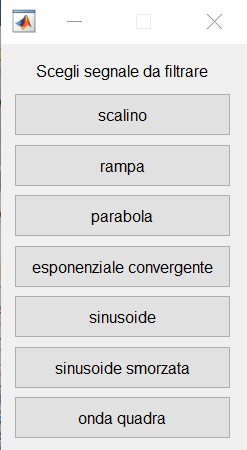
\includegraphics[width=0.38\textwidth]{mainfilterPOSS} 
\caption{Menu di scelta dei segnali}
\end{wrapfigure}
All'inizio dello script vengono definiti il tempo di campionamento e la durata della simulazione in secondi.\\
Viene poi visualizzato un menu che permette di scegliere la natura del segnale da filtrare; i segnali possibili sono tutti e soli quelli ottenibili come uscite da sistemi lineari.\\
I modelli dei generatori di segnale utilizzati vengono riportati nella sezione successiva.
Cliccando uno dei segnali il programma provvederà alla creazione del modello del generatore ed alla sua successiva discretizzazione attraverso le funzioni \textit{built-in} di \textit{MATLAB}.
\begin{lstlisting}[frame=single]
sys = ss(A,B,C,D);
sysd = c2d(sys,dt); 
[Ad,Bd,Cd,Dd] = ssdata(sysd);
\end{lstlisting}
Successivamente vengono definite le matrici di covarianza dei rumori di processo e misura. I valori di tali matrici possono essere variati per aumentare o diminuire la rumorosità del segnale da filtrare.
\begin{lstlisting}[frame=single]
Q=1e-3;
R=1e-1*eye(p);
\end{lstlisting}
Vengono a questo punto inizializzati gli oggetti relativi al generatore di segnale e al filtro di Kalman e si definisce il ciclo che esegue la simulazione.
\begin{lstlisting}[frame=single]
% inizializzazione sistema generatore di segnale rumoroso
sys=sistema(Ad,Bd,Cd,Dd,W,Q,R,x0);

% inizializzazione filtro di kalman
P0=eye(n);
k=filtrokalman(Ad,Bd,Cd,Dd,W,Q,R,zeros(n,1),P0);
\end{lstlisting}
\newpage
\begin{lstlisting}[frame=single]
%% simulazione
for i=1:length(t)
	x(:,i)=sys.leggiStato();     % lettura stato sistema (segnale da ricostruire, per plot)
	y(:,i)=sys.leggiUscita();    % lettura uscita sistema (segnale rumoroso)
	sys.update();                % calcolo del nuovo stato del sistema
	k.update(0,y(:,i));          % aggiornamento filtro --> parametri u=0 e y(segnale rumoroso)
	xs(:,i)=k.leggiStima();      % lettura stima kalman
	Lplot(:,:,i)=k.leggiL();     % lettura matrice L per animazione
	Pplot(:,:,i)=k.leggiP();     % lettura matrice P per animazione
end
\end{lstlisting}
Una volta completata la simulazione, viene visualizzato il plot con il confronto tra segnale da ricostruire, campioni rumorosi e segnale ricostruito dal filtro.
Nella stessa finestra viene visualizzata l'animazione delle matrici di covarianza dello stato e del guadagno.\\
Di seguito viene riportato un esempio di filtraggio di un segnale sinusoidale:

\begin{figure}[h]
	\centering
	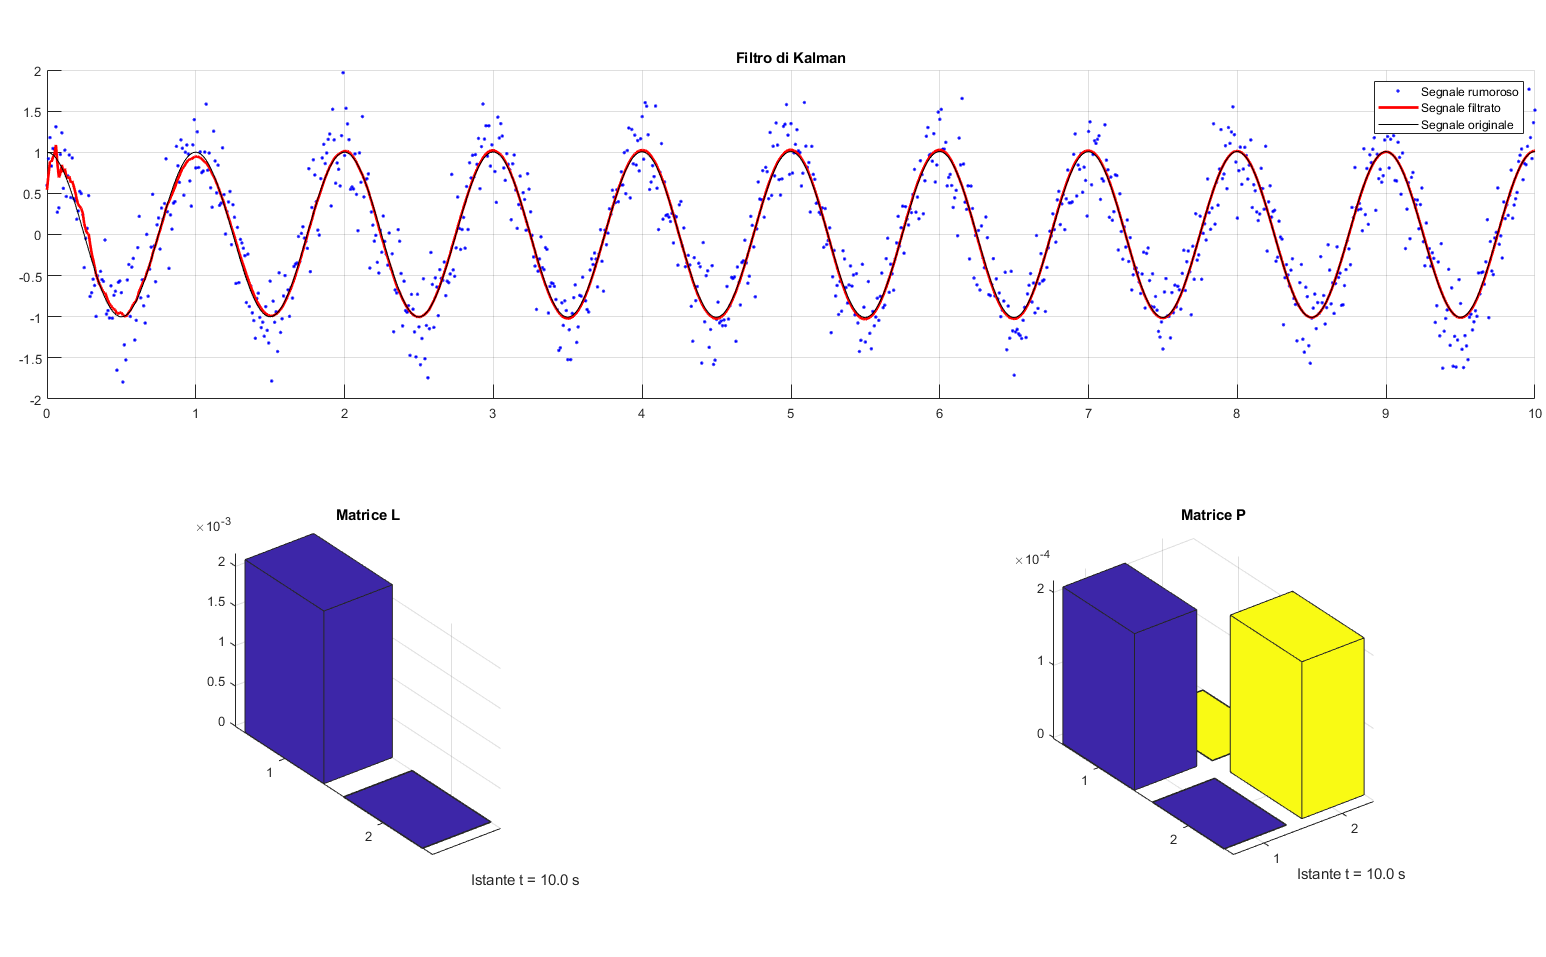
\includegraphics[width=\textwidth]{esempioSinusoide}
\end{figure}

\newpage

\subsection{Modelli dei generatori di segnale}
I generatori di segnale sono sistemi lineari autonomi ($B=0$) ad uscita scalare ($p=1$). La loro evoluzione a partire dallo stato iniziale $x(0)$ genera segnali diversi in base alla natura della matrice dinamica $A$.\\
In particolare il segnale viene prodotto nell'ultima componente dello stato $x(t)$, quindi la matrice di uscita sarà del tipo: $C=\begin{pmatrix}0 & ... & 0 & 1\end{pmatrix}$.\\
Di seguito sono riportati i modelli utilizzati nell'applicazione, che per semplicità sono scritti a tempo continuo e poi discretizzati da MATLAB.
\begin{itemize}
	\item Segnali polinomiali di grado $n$:  
	\begin{equation*}
		x(t)=a_nt^n + ... + a_1t + a_0
	\end{equation*}
	\begin{equation*}
		A=\begin{pmatrix}
		0 & 1 & 0 & ... & 0\\
		0 & 0 & 1 & ... & 0\\
		\vdots & & & \ddots &\\
		0 & 0 & ... & 0 & 1\\
		0 & 0 & ... & 0 & 0
		\end{pmatrix} \in \mathbb{R}^{(n+1) \times (n+1)}, \qquad x(0)=\begin{pmatrix}a_0 \\ a_1 \\ ... \\ a_n\end{pmatrix}
	\end{equation*}
	\begin{itemize}
		\item Scalino  ($n=0$): $A=0$
		\item Rampa    ($n=1$): $A=\begin{pmatrix}0 & 1\\0 & 0\end{pmatrix}$
		\item Parabola ($n=2$): $A=\begin{pmatrix}0 & 1 & 0\\0 & 0 & 1\\0 & 0 & 0\end{pmatrix}$
	\end{itemize}
	\item Segnale esponenziale:
		\begin{equation*}
		x(t)=x_0e^{\alpha t}
		\end{equation*}
		\begin{equation*}
		A=\alpha \in \mathbb{R}, \qquad x(0)=x_0
		\end{equation*}
	\item Segnale sinusoidale ad ampiezza costante:
		\begin{equation*}
		x(t)=a\cos(\omega t)
		\end{equation*}
		\begin{equation*}
		A=\begin{pmatrix}0 & -\omega\\ \omega & 0\end{pmatrix} \in \mathbb{R}^{2 \times 2}, \qquad x(0)=\begin{pmatrix}a \\ 0\end{pmatrix}
		\end{equation*}
	\item Segnale sinusoidale smorzato:
	\begin{equation*}
	x(t)=ae^{\alpha t}\cos(\omega t)
	\end{equation*}
	\begin{equation*}
	A=\begin{pmatrix}\alpha & -\omega\\ \omega & \alpha\end{pmatrix} \in \mathbb{R}^{2 \times 2}, \qquad x(0)=\begin{pmatrix}a \\ 0\end{pmatrix}
	\end{equation*}
\end{itemize}

\newpage